\chapter{Pre-Requirementsuration Setup}
%Intro\footnotemark\\
\begin{spacing}{1.2}
%note en bas de page
\section{Openstack Victoria}

\par The installation of centos-release-openstack-victoria, rabbitmq-server and memcached is done via dnf. A
After installation is complete, an update of the CentOS System is required. 
\\
\begin{figure}[!htb] 
\begin{center} 
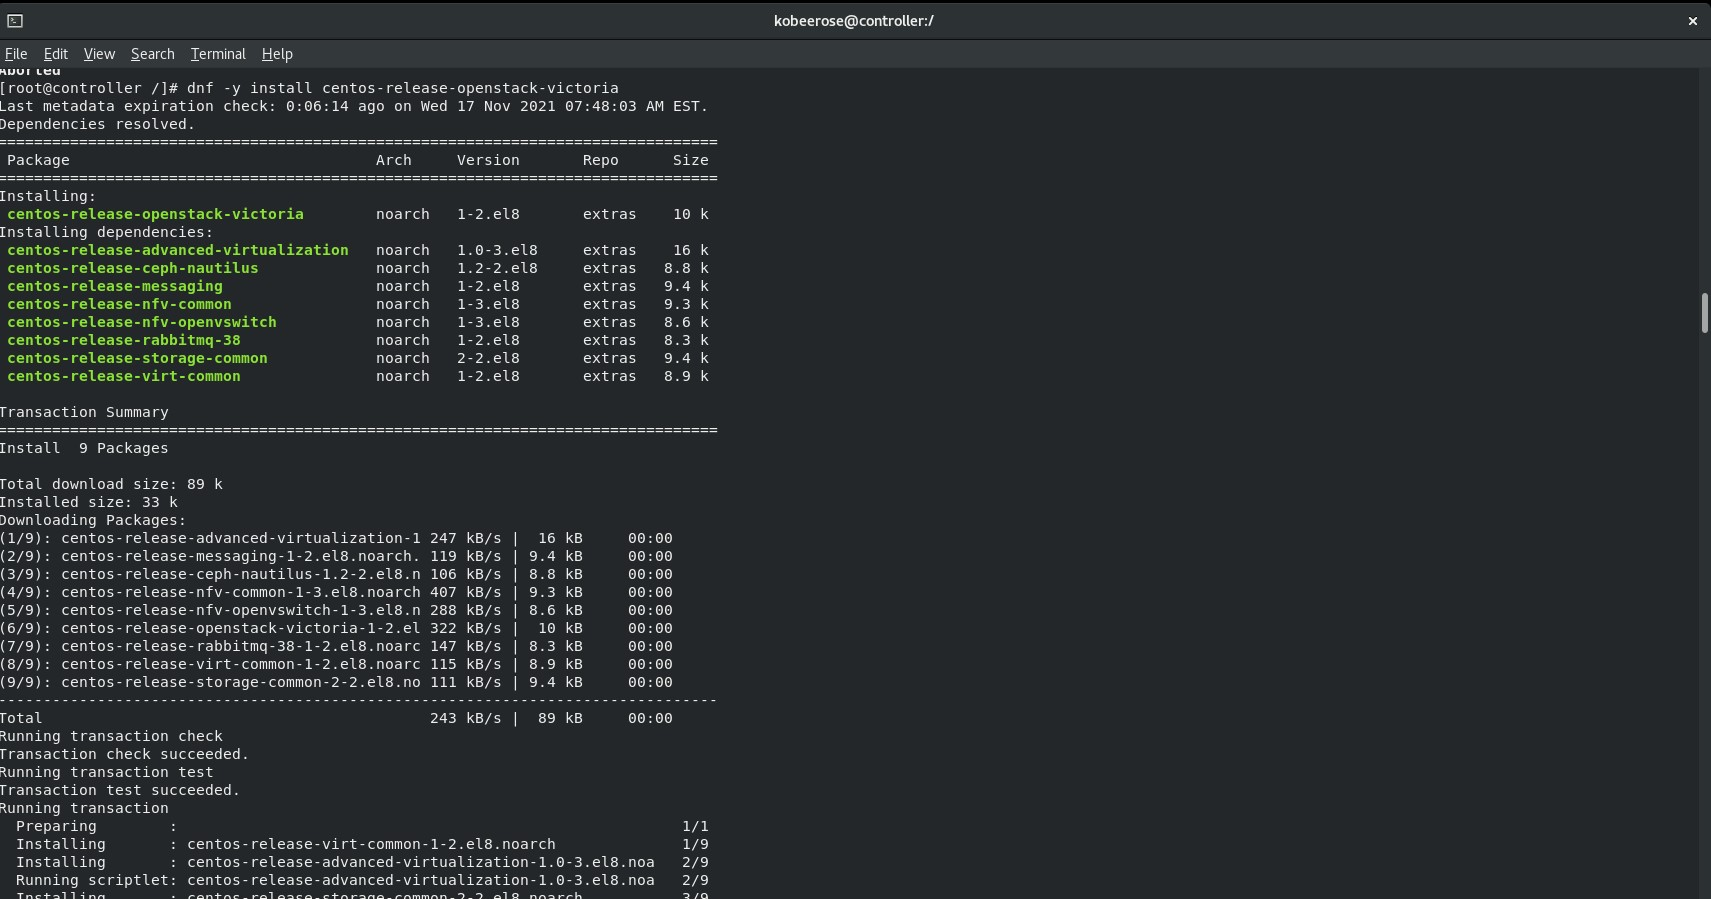
\includegraphics[width=1\linewidth]{Cloud/Pre-Requirements/Installing openstack-victoria} 
\end{center} 
\caption{Installing openstack-victoria} 
\end{figure}  \FloatBarrier
\\
\\
\begin{figure}[!htb] 
\begin{center} 
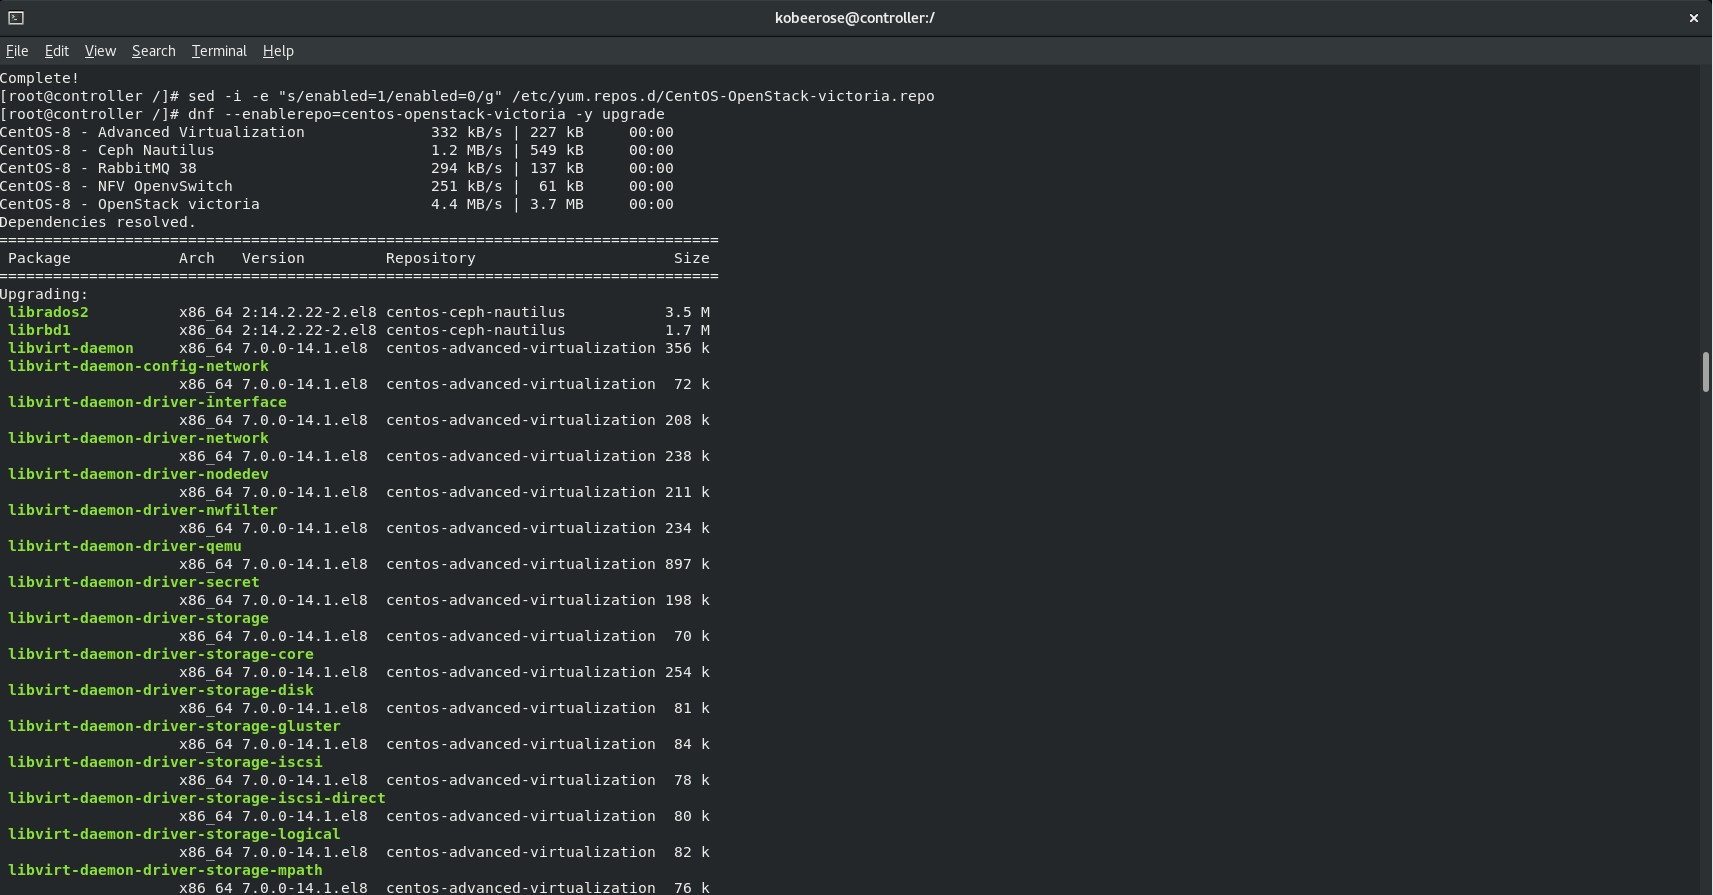
\includegraphics[width=1\linewidth]{Cloud/Pre-Requirements/Add Openstack Repo _ Upgrade CentOS System} 
\end{center} 
\caption{Add Openstack Repo _ Upgrade CentOS System} 
\end{figure}  \FloatBarrier
\\

\section{Installation of RabbitMQ, Memcached.}

\par First of all we need to install RabbitMQ server
\\
\begin{figure}[!htb] 
\begin{center} 
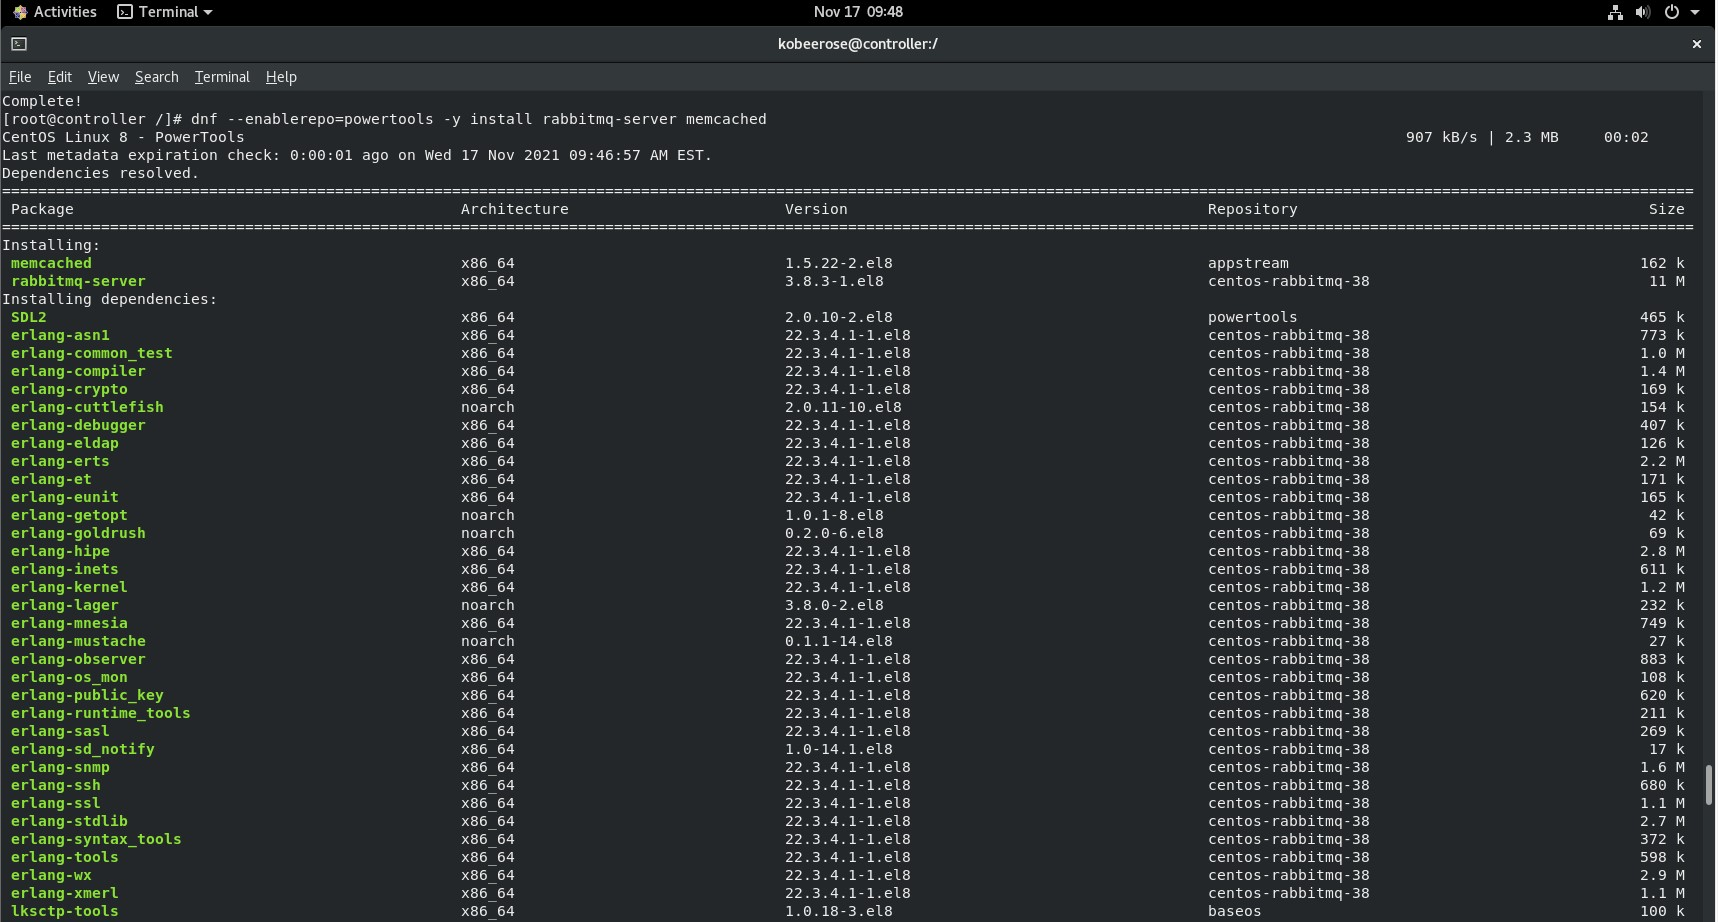
\includegraphics[width=1\linewidth]{Cloud/Pre-Requirements/Installing rabbitmq-server} 
\end{center} 
\caption{Installing rabbitmq-server} 
\end{figure}  \FloatBarrier
\\
\par We are going to change in the file /etc/my.cnf.d/mariadb-server.cnf the default value 151
which is not sufficient in the Openstack environment. And to consider the modifications, we
let's restart and enable mariadb rabbitmq-server and memcached. 
\\
\begin{figure}[!htb] 
\begin{center} 
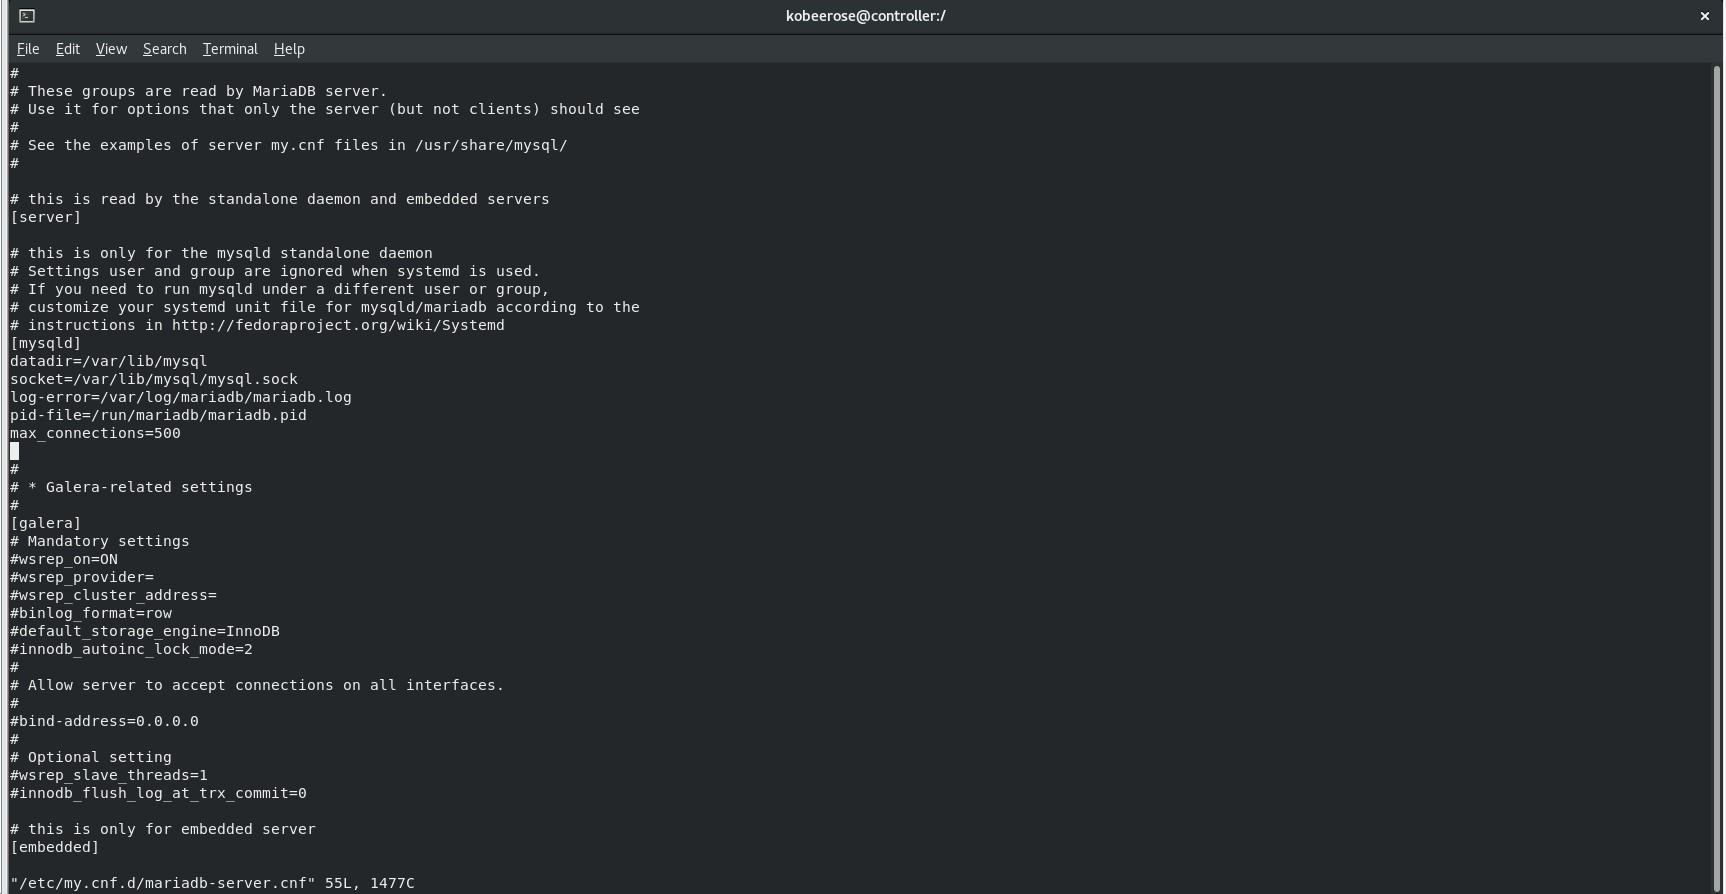
\includegraphics[width=1\linewidth]{Cloud/Pre-Requirements/changing max_connections} 
\end{center} 
\caption{changing max_connections} 
\end{figure}  \FloatBarrier
\\
\par now we persue with configuring the memcached file in order to listen to all
\\
\begin{figure}[!htb] 
\begin{center} 
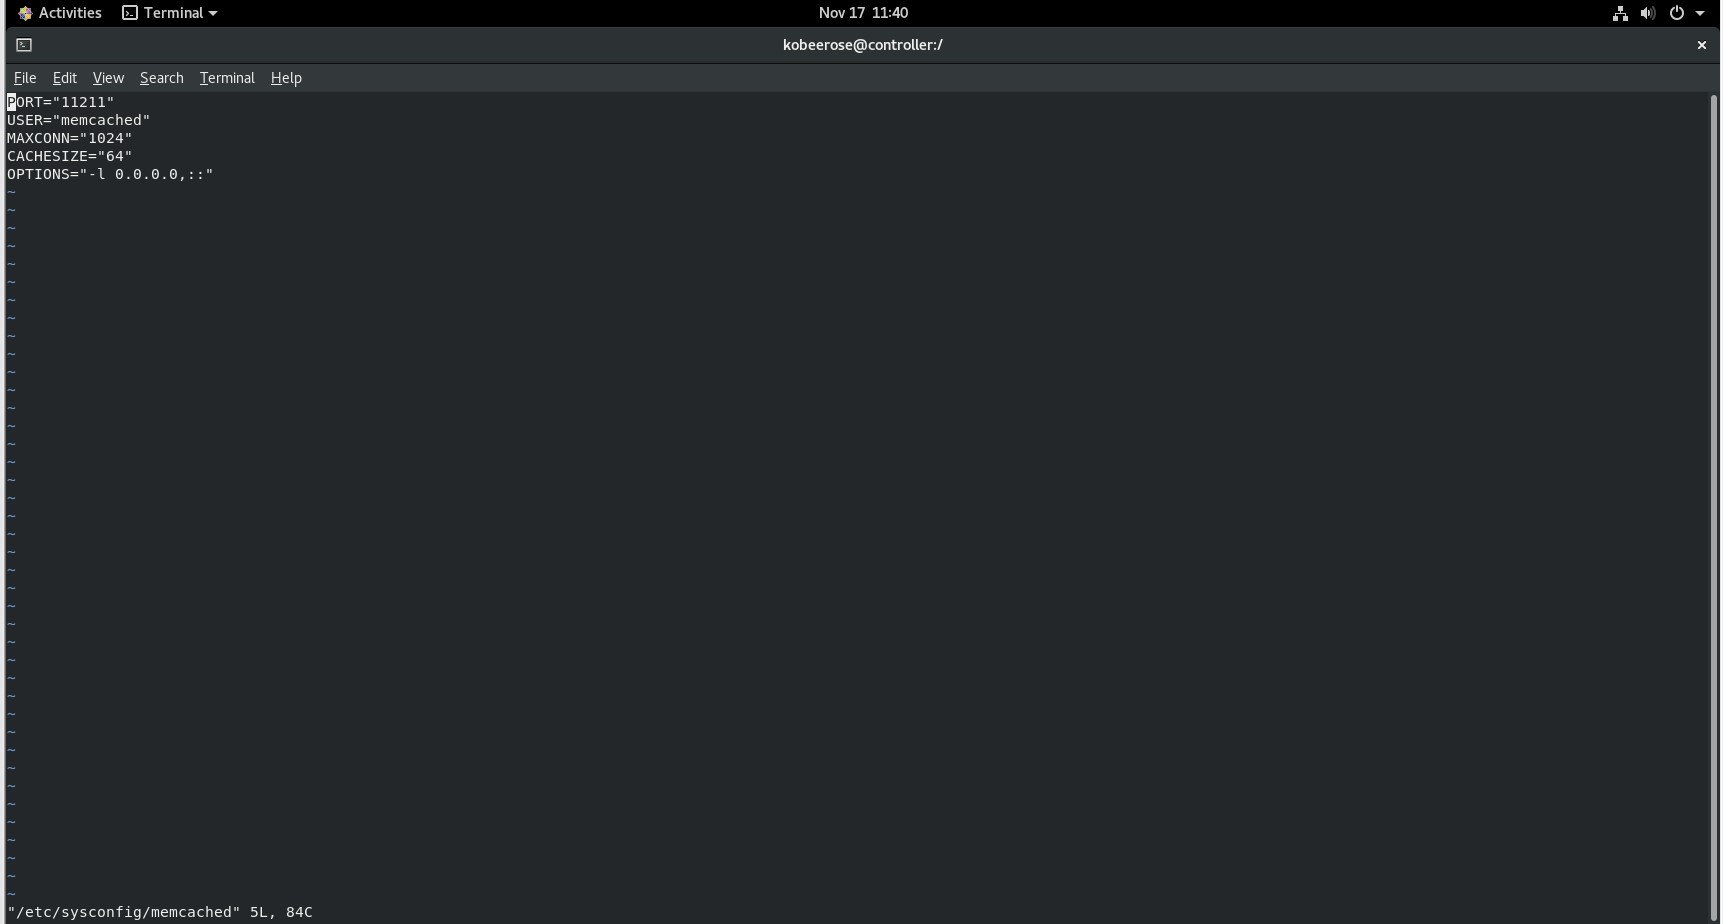
\includegraphics[width=1\linewidth]{Cloud/Pre-Requirements/memcached config} 
\end{center} 
\caption{memcached config} 
\end{figure}  \FloatBarrier
\\
\section{rabbitmqctl config }
\\
\par After that, we will add a new openstack user, define a password for him.
, also give it all the permissions and if SELinux is enabled, we have to change the policy
via a rabbitmqctl.te file and We will use the checkmodule and semodule commands to verify and compile this module.
of SELinux security policy in a binary representation8 
\\
\begin{figure}[!htb] 
\begin{center} 
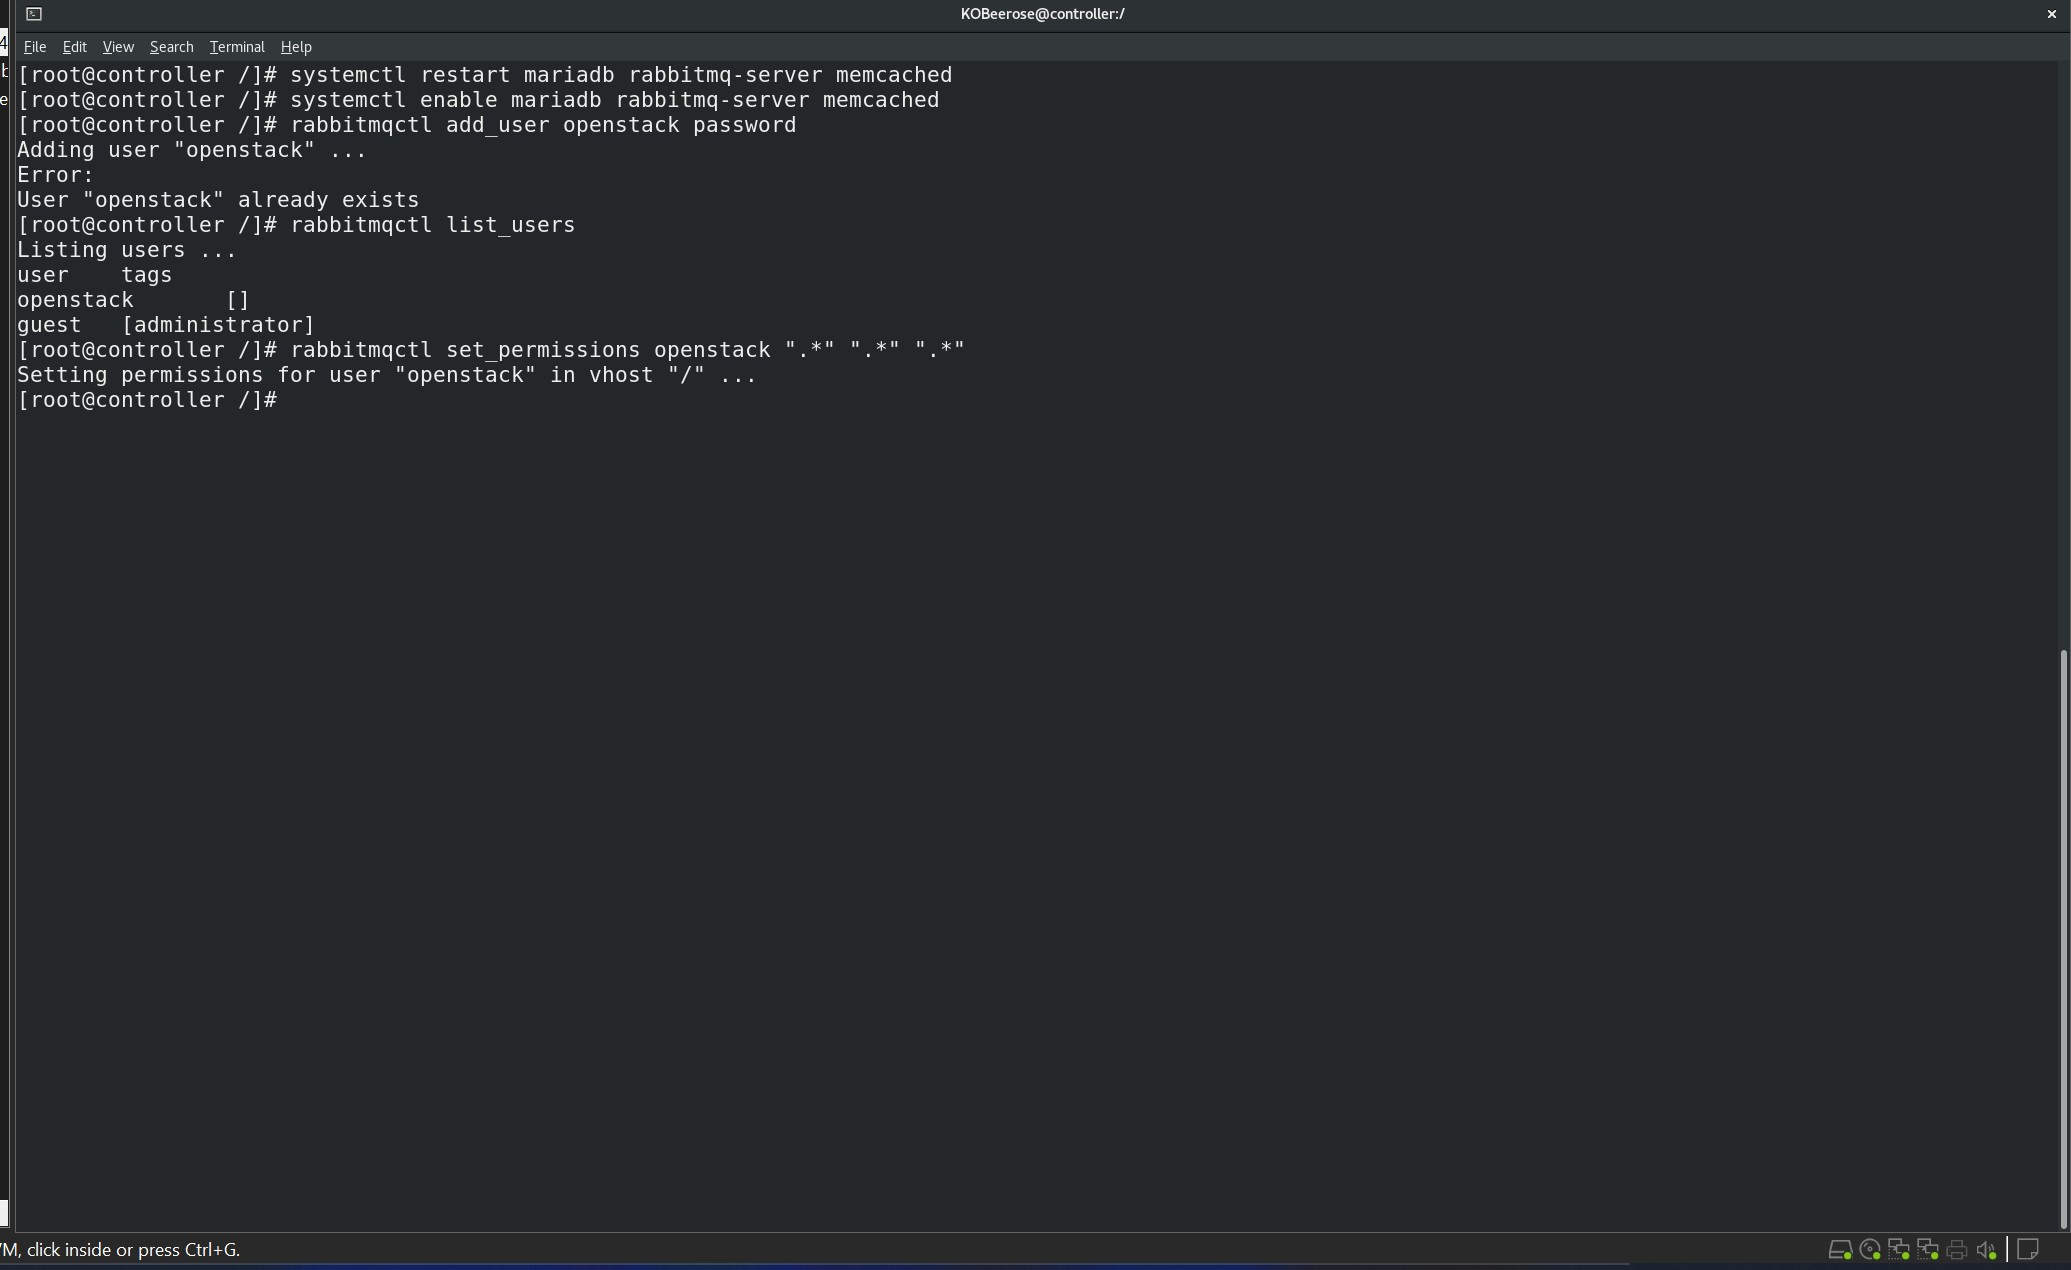
\includegraphics[width=1\linewidth]{Cloud/Pre-Requirements/Creating a new openstack user} 
\end{center} 
\caption{Creating a new openstack user} 
\end{figure}  \FloatBarrier
\\


\par Allowing mysql service, the port 5672 service and reloading the firewall.\\
\\
\begin{figure}[!htb] 
\begin{center} 
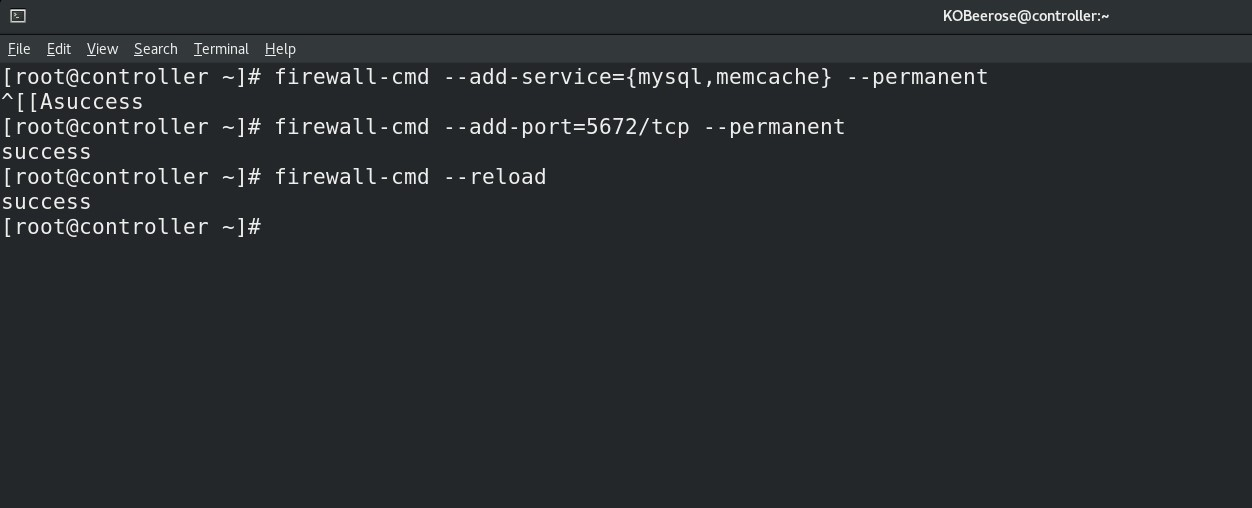
\includegraphics[width=.8\linewidth]{Cloud/Pre-Requirements/Allowing ports for services.} 
\end{center} 
\caption{Allowing ports for services.} 
\end{figure}  \FloatBarrier
\\


\end{spacing}